\chapter{INTRODUCTION}
\label{intro}

This thesis presents a series of experiments searching to define an ideal
execution environment for Software Defined Networking (SDN) applications. By
exploring the different implementation methods utilized in the domain of SDN,
namely pure software and hardware, the benefits and deficits of each be
evaluated and contribute towards a concrete specification. In a pure software
implementation, most all of the underlying hardware components have been
abstracted, providing more flexibility and compatibility at the cost of
performance. A pure hardware implementation will translate a high level
language into optimized native instructions to keep performance high, but
narrows the set of languages supported. In Figure \ref{overview}, the spectrum
for these two methods is shown.

\begin{figure}[h]
\centering
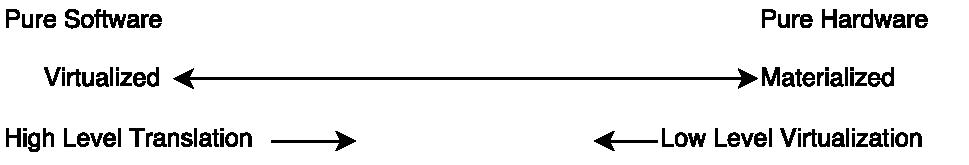
\includegraphics[scale=0.75]{spectrum_base}
\caption{Execution environments for SDN applications can utilize a high level
and low level implementation methods. The sweet spot lies somewhere between
the two.}
\label{overview}
\end{figure}

To translate high level code to a target device's native instruction set, more
work has to be done by the compiler to support both the language and the
device. Knowledge of the targets architecture, including specialized hardware
accelerators, must be well defined in order optimize execution. However this
approach is not always ideal, especially in the domain of SDN where network
switch architecture varies greatly between vendors in terms of capabilities
and features. This contributes to a lack of generalization in modern networking
where end-users are typically only able to specify configuration settings. In
order to bridge the gap, hardware components can be abstracted to provide
low level access to resources available in the system. A suitable execution
environment would lie somewhere between these two, taking advantage of powerful
compilers that can lower high level code while also leveraging low level
resource interfaces raised from the hardware.

\section{Background}
\label{intro:bg}
Networking architecture has become the focus of many facets in computing with
an increased reliance on network data. As more and more devices become
connected and users produce and consume data at an ever-increasing rate, the
way we accommodate these needs in networking infrastructure has prompted the
need for change. In order to service the needs of users, network engineers
require more functionality from their equipment than basic switching and
routing. Their networks need to be more intelligent, and allow for more
powerful user generated network applications. Unfortunately conventional
network switching devices are fairly static and rigid, and do not provide the
means to network engineers to create custom applications that suit their
particular needs. A network switch is composed of two high level components, a
control plane and a forwarding, or data, plane. The control plane manages the
configuration and state of the device, as well as compiled application
tenancy; whereas the data plane is responsible for executing forwarding
behavior over network traffic flows in the system. These components are
tightly coupled which hinders how a network application might be able to
abstract their functionality. At the upper level, control plane management is,
more or less, a fairly open entity. Users can configure their networks and
applications running on them within the confines of the interface exposed by
that particular switch vendor. To apply changes made in the control plane,
which may alter the configuration of the data plane, usually the device must
be rebooted. Most changes made to resources used by the data plane and
applications can only occur when the system is starting up. This has much to
do with the fact that the applications running on these devices are created by
the vendors themselves, who understand the underlying architecture in the
system and are able to push the application logic down into the hardware. The
result is high performance networking applications, that utilize hardware
accelerators and are tuned for that particular system. However this comes at a
great cost, flexibility. Network engineers are at the mercy of networking
device manufacturers when they want to mold their network to suit their needs.
The data plane in a network switch remains a black box, with features and
capabilities varying greatly between vendors. This lack of transparency makes
it difficult to model an abstract machine that can be targeted by networking
applications.

Research in the domain of SDN investigates the
decoupling of the two planes, giving users the ability to create networking
applications that can respond to changes in network traffic flows in real time.
The emphasis in this model is to allow a single control plane to manage
numerous data planes in one or many switches as a unified entity. Most of the
work in this field revolves primarily around virtual network switches,
building on concepts provided by the OpenFlow specification \cite{openflow}.
We chose to focus on the implementation of a single programmable network
device, where the control and data plane exist within the same system. This
allowed us to produce a specification for an abstract machine for networking
applications. The machine defines memory and object models, program execution
semantics, a set of required operations, access to guaranteed resources, and
the types of objects that it operates on and their behaviors. It must also be
able to support a variety of high level programming languages as well as
platforms and network processor architectures. Optimization support for
specialized instruction execution and offloading computation to hardware
accelerators and/or co-processors is also a key requirement to keep
performance on par. Languages are able to interact with the virtual machine
through an application binary interface (ABI), that defines symbols and rules
that dictate how they can utilize the runtime system. This approach has
produced an instance of an abstract machine that provides the necessary
resources and capabilities required to support network application execution.


\section{Goals}
\label{intro:goals}
It is clear that there is need for runtime support for compiled
networking applications. The virtual machine needed to provide functionality
for both parts of a network switch, the control and data planes, and allow
applications to have control and access to these resources at the user level.
In addition to servicing the needs of applications, the runtime needs to be
supported on a variety of architectures and utilize the materialized and
abstracted resources available. Freeflow aims to fill the gap between high level network
programming langauges and low level switch architectures for the purpose of SDN.

\section{Contributions}
\label{intro:contrib}
The contributions presented in this thesis come from numerous experiments with
low level networking hardware. These experiments helped characterize the
problem domain with respect to low level abstraction of network interfaces and
high level language translation to a native instruction set architecture
(ISA). The experiments evaluated include:

\begin{itemize}
  \item DPDK - Low level port abstractions
  \item Netmap - Low level port abstractions
  \item RISC-V - Native instruction execution
\end{itemize}

% \subsection{Virtual Machine}
% \label{intro:vm}
% FFVM is a process that provides the resources necessary for network
% applications to execute. These resources are:
%
% \begin{itemize}
% \item \emph{Ports} - The source of I/O for applications.
% \item \emph{Tables} - Matching data structures that define forwarding behavior.
% \item \emph{Packet Context} - Contextual information about a packet.
% \item \emph{Action Exection} - Native FFVM instructions to be executed by the
% runtime.
% \item \emph{Memory} - Packet Context buffers.
% \item \emph{Threading} - Infrastructure for modeling applications in various
% threading architectures.
% \end{itemize}
%
% \subsection{Runtime Support Library}
% \label{intro:rsl}
% Freeflow provides a runtime support library that Steve applications can
% leverage to execute as efficiently as possible. The library houses a collection
% of system calls, exposed as external C functions, to allow applications to call
% into the system during execution. These system calls allow the runtime to map
% the execution of certain instructions to the most appropriate computational
% device present and provide access to guaranteed resources.

\section{Road Map}
\label{intro:map}
% Write a short paragraph about each topic.
This paper covers our initial work towards a fully programmable networking
device. The main topics in this thesis are described in the following
paragraphs.

Related works are contained in the Chapter \ref{related}, detailing some of the
more mature research efforts in the domain of SDN. An explanation of the SDN
paradigm, the OpenFlow protocol, network applications, as well as various
platforms and frameworks considered can be found here.

In Chapters \ref{hardware} and \ref{insn}, the early investigations into
hardware abstraction and processing instructions are discussed,
respectively. This section journals the different approaches that were
considered in the design and implementation throughout this project, and
explains the benefits, deficits, and lessons learned from each approach.

Chapter \ref{ff} covers the design and implementation of the Freeflow system,
including application hosting, the virtual machine, the runtime support
library and the application binary interface exposed. This chapter discusses
the details of the contributions made towards this work at length.

Chapter \ref{expr} presents the experiments conducted as well as some initial
evaluation metrics collected. These demonstrate basic networking device
functionality for emulating Ethernet port end-points and cross-connects over
TCP sockets, and provide a baseline which can be used to further optimize the
system.

In the final chapter, Chapter \ref{concl}, the conclusions drawn from the
research conducted are laid out. Future work for this project is also discussed
in this chapter.

Lastly, Appendix \ref{abi-listing} contains a listing of the ABI provided by
the Freeflow virtual machine as a reference.
